\documentclass[a4paper,11pt]{article}
\usepackage[utf8]{inputenc}
\usepackage{amsmath}
\usepackage{amsfonts}
\usepackage{amssymb}
\usepackage{graphicx}
\usepackage[backend=biber]{biblatex}

\addbibresource{nn.bib}
\renewcommand\thesubsection{\alph{subsection}}


%opening
\title{Computational properties of neural columns arising from temporal dynamics}
\author{Vince Baker, advisor: Dr. Luis Cruz Cruz\\ Drexel University Department of Physics}

\begin{document}

\maketitle

\begin{abstract}
We investigate the computational properties of a neural column structure using the Liquid State Machine (LSM) paradigm.
We enhance the neural model used in the original LSM work to incorporate more realistic neuron dynamics and action potential propagation delay.
The enhanced model shows synchronous wave propagation behavior with propagation speed that depends on the column width. 
The column encodes information about the input spike trains in its dynamic state as required for LSM processing.

\end{abstract}

\section{Introduction} 
 The human brain hosts advanced cognitive processes that remain only partially understood.
Computational neuroscience seeks to understand brain functions through modeling at several levels of physical fidelity.
``Biologically inspired'' computation models are used in machine learning to solve a variety of problems that are intractable with conventional approaches.
Computational biophysics provides insight into the lowest levels of neural functions while nonlinear dynamics provides tools for understanding some aspects of cognition.
This research will explore the computational properties of neural networks through a novel combination of biophysics, nonlinear dynamics and machine learning.
\\
In the machine learning community network models are developed and trained to solve specific problems, with the trained networks then graded against data sets representing those specific problems.
These computational network models include multi-layer perceptrons, feed-forward "convolutional" networks, and recurrent networks with memory.
These models have been effectively applied to solve diverse problems including image recognition and classification, speech recognition and handwriting recognition.
The common computational models may be considered biologically-inspired, but none of them are biologically plausible.
All of these approaches greatly simplify the network and synapse dynamics.
Multi-layer perceptrons and feed-forward networks do not include recurrent connections, and are trained through biologically unrealistic methods involving back-propagation of error terms.
Recurrent network models such as long short-term memory (LSTM)  incorporate feedback with a basic concept of memory, but the dynamics and training mechanisms are still not biologically plausible.
\\ \\
In this work we adapt the more biologically plausible Liquid State Machine (LSM) model first developed in \cite{maas2002} and shown in figure \ref{fig:lsm_structure}.
In the LSM model a recurrently connected network, called the liquid or the reservoir, is excited with a time-varying input.
The stimulus perturbs the liquid and creates a complex state progression like pebbles dropped into a pond.
The time history of the input is encoded into the liquid state through the recurrent connections.
A trained readout network then decodes the desired information from the liquid state. 
The recurrent connections in the liquid create a fading memory property so that the time history of the input becomes encoded in the liquid state.
Figure \ref{fig:lsm_memory} from \cite{maas2002} shows that a liquid state machine can recognize segments of a spike train that occurred up to 750 milliseconds in the past using only the current state of a liquid network.
\\
The LSM model has unique features that make it biologically plausible. 
The large liquid network can be randomly connected and does not need to be trained.
The readout network can be trained with biologically plausible Hebbian learning and does not require error backpropagation \cite{auer2002}.
Multiple independent readout networks can be trained to simultaneously extract different information from the same liquid network (figure \ref{fig:lsm_multiple_readouts}).
Liquid state machines have also proven an effective computational model, achieving world-class results in speech recognition \cite{zhang2015}.
\\ \\
Two important properties of the liquid state machine are the separation property and the approximation property.
The separation property reflects the distance between liquid network trajectories (time-evolved states) induced by different inputs.
The separation property is mostly a function of the liquid itself.
The approximation property addresses the ability of the LSM to decode the desired information from the trajectory of the liquid.
The approximation property depends mostly on the particular structure and adaptation mechanism of the readout layer.
\\ 
To characterize the separation property of their liquid network Maas and Markram injected various spike trains and observed the resulting liquid states.
They defined the distance between two spike trains by correlating the spike trains against each other.
This definition is valid for closely related spike trains that may only differ by a translation in time.  
Improved distance metrics have been developed that are timescale-independent and time-resolved including inter-spike interval (ISI) and SPIKE \cite{kreuz2012}.
The SPIKE metric in particular provides an improved time-resolved distance metric across time scales and time shifts.

\section{Methods}
We re-examine the neural column circuit used as an LSM liquid network in \cite{maas2002}.
In this work we explore the additional temporal dynamics found in realistic neural structures.
We adopt a more realistic model for neuron dynamics that allows us to explore the rich variety of behaviors found in biological neurons.
We also incorporate action-potential propagation times that are proportional to the physical distance between neurons.
The dynamics of a small neural column are then simulated under various conditions to explore neuron synchronization, effective propagation velocity and the transformation properties of the column.
Our model provides simulation of important physical parameters and constructs while still remaining computationally tractable for machine learning tasks such as pattern recognition on large data sets.
\\
In their original work Maas and Markram used a simple integrate-and-fire neuron model combined with a sophisticated synapse model first presented in \cite{markram1998}.
Their neural column was composed of 135 neurons on a unit column, 3x3 neurons wide and 9 neurons high as shown in figure \ref{fig:column_structure}.
The neurons were connected according to a distance-based rule:
\begin{align}\label{eq:connectivity}
 P_{a,b} &= C \times e^{-(D(a,b)/\lambda)^2}
\end{align}
80\% of these neurons were excitatory, 20\% of the neurons were inhibitory. 
The transmission delays between neurons were fixed to 1.5 ms for excitatory-excitatory connections and 0.8 ms for all other connections.
The synaptic responses were modeled using the dynamic model in \cite{markram1998}. \\
This model, although highly simplified, incorporates many biophysical parameters.
The recurrent connections, general structure, connectivity and synaptic dynamics are all higher fidelity than a typical computational model.
The authors were able to directly measure the effects of certain parameters using a variety of computational tasks including spiking rate estimation, pattern recognition, spike coincidence and spatial distribution. 
For example, the best performance on a spike pattern classification task was achieved with $\lambda=2$ in equation (\ref{eq:connectivity}) (figure \ref{fig:lambda_performance}).
\\
Computational neuroscientists, biophysicists and machine learning researchers use various models to simulate neural networks (figure \ref{fig:neural_models}).
Most liquid state machine implementations have used simple integrate-and-fire neurons due to their low computational complexity.
We have chosen the Izhikevich model \cite{izhikevich2003} to allow us to explore the neural dynamics.
The Izhikevich model uses two coupled differential equations with two variables and four parameters:
\begin{align}
 v^\prime &= 0.04v^2+5v+140-u+I\\
 u^\prime &= a(bv-u)\\
 \text{if } &v>30: v\leftarrow c, u\leftarrow u+d
\end{align}
This is a simplified model of a two-dimensional dynamical system.
This model has been used to reproduce common neural firing patterns (figure \ref{fig:izzy_model}). \\
We enhanced the available MATLAB code for the Izhikevich model to incorporate propagation time between the neurons through the use of a delay buffer.
This allowed us to study the temporal effects of action potential propagation time.
\section{Results}
We first verified that our enhanced model reproduced the qualitative behavior of the original Izhikevich model for the same parameter settings.
Our test simulation was based on the MATLAB simulation available at (\cite{izzy_code}).
The simulated neural circuit had a pool of 1000 neurons, with 800 of the neurons (80\%) excitatory and 200 (20\%) inhibitory.
The Izhikevich parameter ``a'' was 0.02 for excitatory neurons and uniformly drawn from 0.02-0.10 for excitatory neurons.
The parameter ``b'' was 0.2 for excitatory neurons and uniformly chosen from 0.2-0.25 for inhibitory neurons.
The parameter ``c`` was -65 for inhibitory neurons and randomly chosen from -65 to -50 for excitatory neurons.
The parameter ''d`` was was 2 for inhibitory neurons and uniformly chosen from 2-8 for excitatory neurons.
All neurons were completely connected with synaptic strengths of 0-0.5 for excitatory connections and -1 to 0 for inhibitory connections.
A continuous random input was applied to all neurons, drawn uniformly from 0-5 for excitatory neurons and 0-2 for inhibitory neurons.
We ran simulations using the original Izhikevich code as well as our modified code with synaptic propagation delays.
The spike patterns are shown in figure \ref{fig:izzy_enhanced}.
The same partially-synchronized firing is shown to occur in both simulations. 
This validates our implementation of the Izhikevich model with propagation delays.
\\ \\
We next explored the effect of our distance-dependent propagation times on the dynamics of a neural column.
To test the effect of the distance-dependent propagation times we created two columns, 3x3x40,  with identical neurons and identical connectivity.
The first column has random propagation times, the second column uses distance-dependent propagation times.
The bottom 10 layers were stimulated with the random thalamic input as described above \cite{izhikevich2003}.
The resulting firing patterns are shown in figure \ref{fig:delaycompare}.
The column with random delay shows random firing activity in the stimulated region, but no propagation through the column.
The column with distance-dependent propagation shows correlated firings with a clear propagation down the column.
These results demonstrate that distance-dependent propagation delay can be a critical parameter in the qualitative behavior of a neural circuit.
The wave propagation phenomenon is particularly interesting in the context of \cite{keane2015} where similar propagating waves arose from random input in a two-dimensional neural circuit.
The authors in \cite{keane2015} propose these propagating waves as a mechanism for synchronizing a network of fundamentally irregular neurons. 
\\
To further explore the temporal dynamics we simulated columns with different shapes. 
Columns with widths of 2, 3 and 4 neurons were constructed with 15 layers each, resulting in total neuron counts of 60, 135 and 240 neurons.
The neurons were 80\% excitatory and 20\% inhibitory with neuron parameters as described above. 
The bottom layer of neurons was stimulated with a 30 mV stimulus for a duration of 10 ms. 
The effective propagation time of the wave packet was measured from the onset of the stimulus until the first firing of a neuron in the topmost layer.
The propagation times for 100 trials are shown in figure \ref{fig:propagation_time}.
The narrow columns have a longer effective propagation time.
This demonstrates that spatial organization of the column structure influences the temporal properties of the neural circuit.
\\ \\
Our final investigation of the column properties characterized the separation property for use in a liquid state machine using the distance metrics from \cite{maas2002}.
We simulated a 3x3x9 column with 135 neurons with the parameters described above.
We created pairs of random Poisson spike trains with a firing rate of 30 Hz.
The individual spikes had a Gaussian shape with $\sigma=4$ ms.
The paired spike trains were then injected into two identical columns.
The spike trains were injected onto 30\% of the neurons in the column chosen at random.
The input synaptic weights were drawn from a Gaussian distribution with mean 1 and standard deviation 1.
Identical injection sites and synaptic weights were used for both columns. 
A typical stimulus and response are shown in figure \ref{fig:reservoir_response}.\\
The distance between each pair of spike trains was measured using the $L_2$ norm.
The distance between the resulting trajectories was also measured using the $L_2$ norm, normalized by the total number of neurons.
From figure \ref{fig:distance} we see that the distance of the neural column trajectories depends on the distance between the input spike trains.
This indicates that a liquid state machine using our modeled column would likely possesses the separation property.

\section{Future work}
The present investigation has created a new model for a liquid state machine that incorporates enhanced neuron dynamics and distance-dependent propagation time.
A neural column simulated using this model has shown synchronized firing and wave packet propagation.
The effective wave propagation time was shown to depend on the thickness of the column.
The separation property of the column was characterized using Poisson spike trains, and it was found that the column encoded the spike train distances into the resulting trajectories.
\\ \\
The current research, as well as previous research by Joseph Tumulty in our group, has found interesting behavior related to relatively slow spike propagation time.
Biological spike velocity varies from about 1 meter/second for unmyelinated axons to  more than 100 meters/second for myelinated axons.
On the millimeter and micrometer length scales of neural circuits this translates to propagation times that are orders of magnitude faster than neuron dynamic time scales.
There are several mechanisms through which slower effective propagation might occur.
\\
In this work we demonstrated that the propagation velocity of a wave through a column structure depends on the spatial properties of the column.
Our research group has previously explored the existence of microcolumn structures, approximately 1 neuron wide, within the larger cortical columns \cite{cruz2000}.
One possible function of these neural microcolumns may be to control wave propagation velocity. 
We will explore this possibility in future work.
\\
Neural dynamics near a bifurcation can result in a delayed firing time \cite{izhikevich}.
This could be another mechanism for slower effective propagation through a neural circuit.
In future work we will examine the behavior of our neural circuits when the neurons dynamics are tuned near to a bifurcation.
\\ \\
In this effort we have demonstrated that a liquid state machine using our neural column would likely possess the separation property.
In future work we will combine our current model with a trained readout map and explore the performance of the resulting liquid state machine.
We will focus on how the liquid state machine performance depends upon temporal dynamics created through neuron parameters and spatial organization.

\section{Figures}
\begin{figure}[p]
 \caption{A liquid state machine consists of a liquid network L and a readout map f. L can be viewed as a nonlinear filter that transforms the input u into a higher dimensional space. The readout map f decodes the desired information from the time-evolving state of L.\cite{maas2002}}
 \label{fig:lsm_structure}
 \centering
   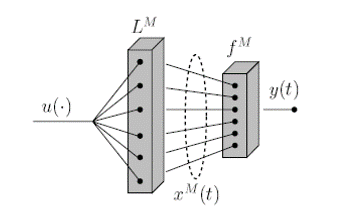
\includegraphics[width=\textwidth]{fig/lsm}
\end{figure}

\begin{figure}[p]
 \caption{A liquid network was stimulated with four sequential 250-millisecond sequences. The readout map was able to identify the first three segments from the liquid state at t=1000 milliseconds if the network included dynamic synapses. \cite{maas2002}}
 \label{fig:lsm_memory}
 \centering
   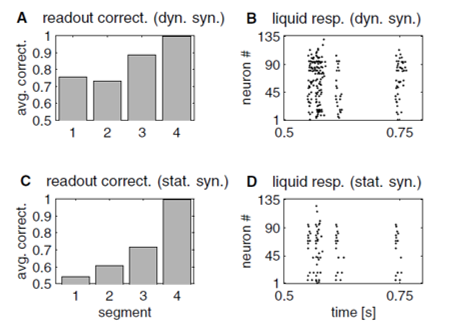
\includegraphics[width=\textwidth]{fig/maas_memory}
\end{figure}

\begin{figure}[p]
 \caption{Column structure used in this research, $\lambda=2$,$C=1$,}
 \label{fig:column_structure}
 \centering
   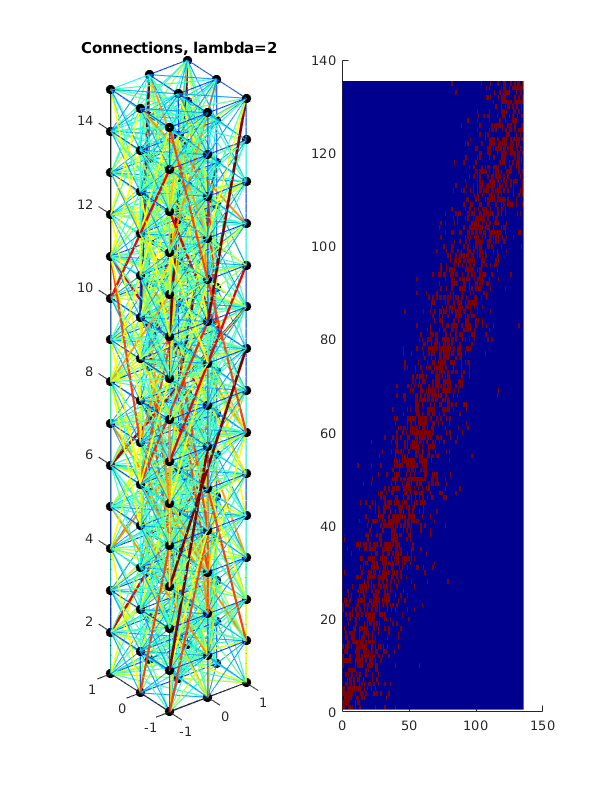
\includegraphics[width=0.48\textwidth]{fig/lambda2}
\end{figure}

\begin{figure}[p]
	\centering
	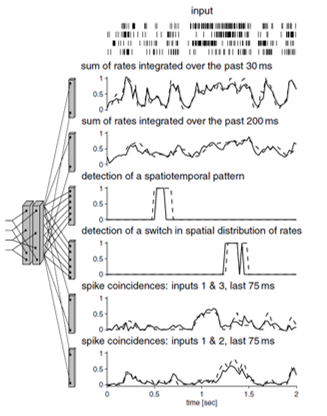
\includegraphics{fig/MultipleReadouts}
	\caption{Multiple readouts from a single reservoir \cite{maas2002}}
	\label{fig:lsm_multiple_readouts}
\end{figure}

\begin{figure}[p]
 \caption{Neural models}
 \label{fig:neural_models}
 \centering
   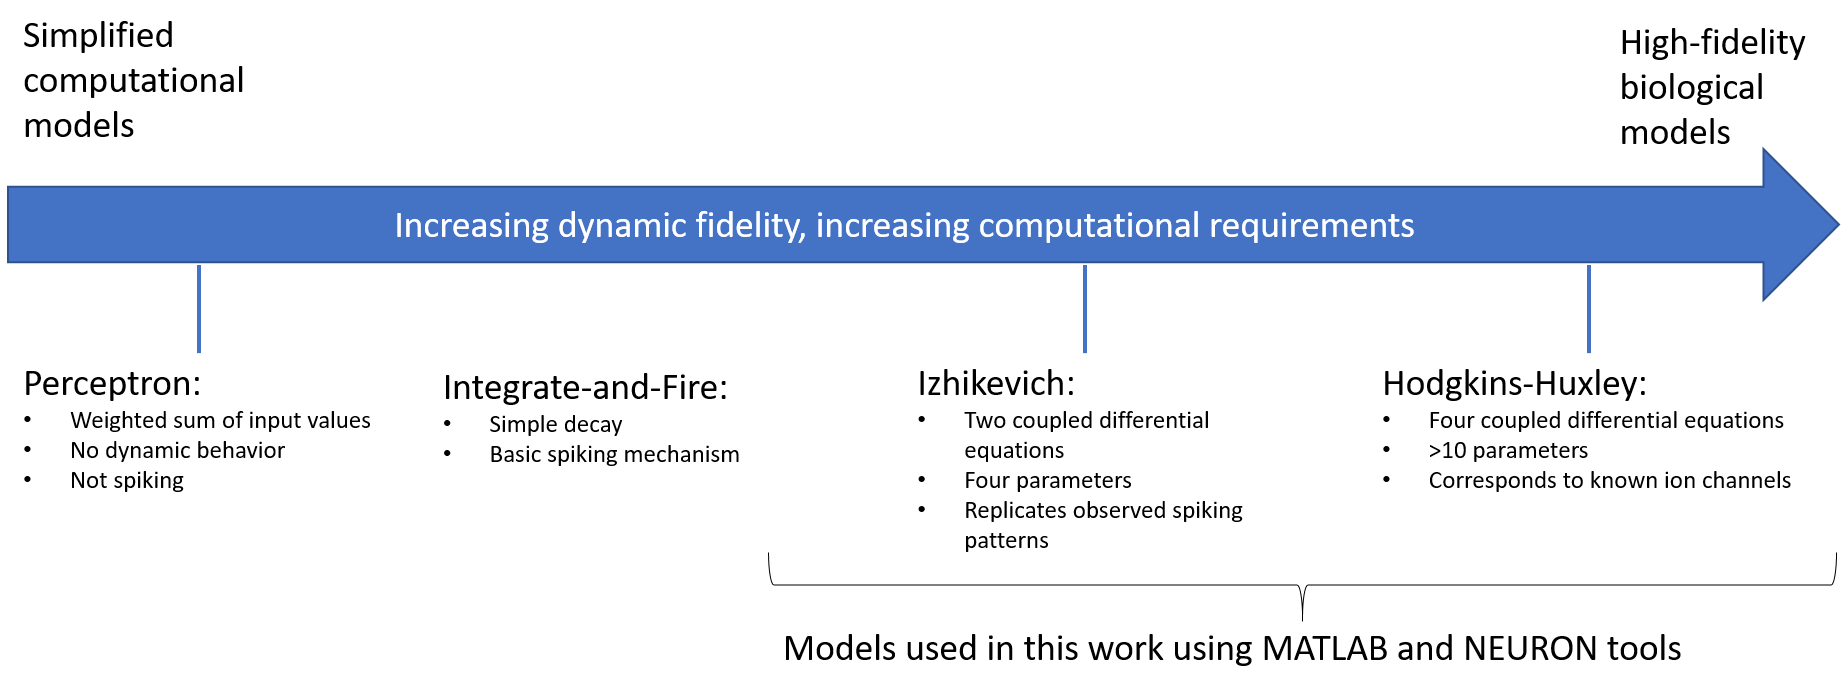
\includegraphics[width=\textwidth]{fig/neural_models}
\end{figure}

\begin{figure}[p]
  \caption{Classification performance from \cite{maas2002}. The best classification performance is acheived with mostly local connectivity with occasional longer connections.}
  \label{fig:lambda_performance}
  \centering
    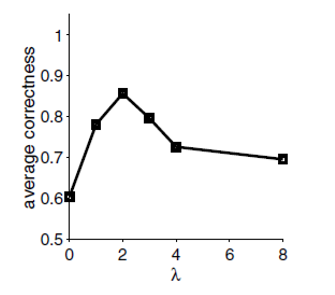
\includegraphics[width=0.48\textwidth]{fig/lambda_performance}
\end{figure}

\begin{figure}[p]
 \caption{The Izhikevich model reproduces common neural firing patterns \cite{izhikevich2003}}
 \label{fig:izzy_model}
 \centering
   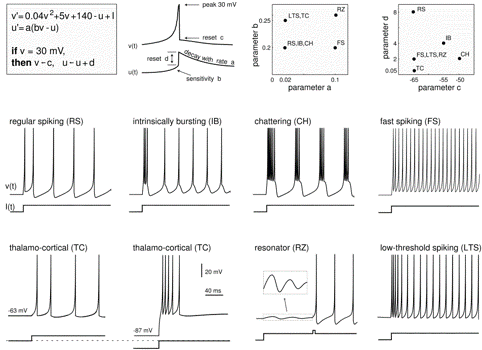
\includegraphics[width=\textwidth]{fig/izzy_model}
\end{figure}

\begin{figure}[p]
 \caption{The original Izhikevich model (left) and our enhanced model (right) with identical parameters with randomized stimulus.}
 \label{fig:izzy_enhanced}
 \centering
   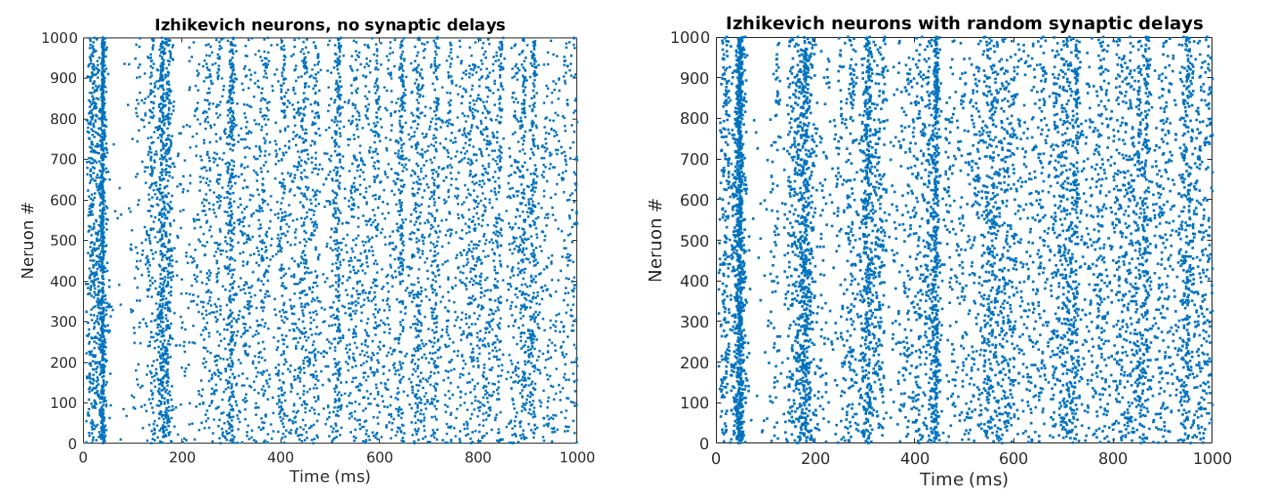
\includegraphics[width=\textwidth]{fig/izzy_enhanced}
\end{figure}

\begin{figure}[p]
 \caption{Two identical neural columns, 3x3x40, with randomized propagation delays (top) and distance-dependent propagation delays (bottom) were stimulated with random input in the first 10 layers,
 The column with distance-dependent propagation delays shows synchronized firing that induce traveling wave packets through the column.}
 \label{fig:delaycompare}
 \centering
   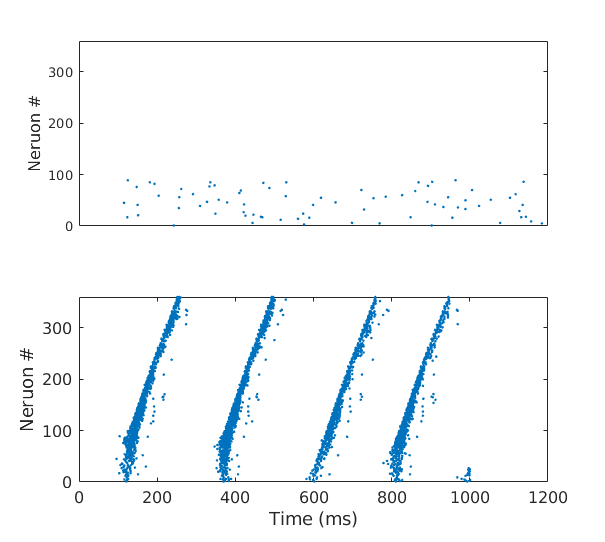
\includegraphics[width=\textwidth]{fig/DelayCompare_RandInput}
\end{figure}

\begin{figure}[p]
 \caption{Effective propagation velocity}
 \label{fig:propagation_time}
 \centering
   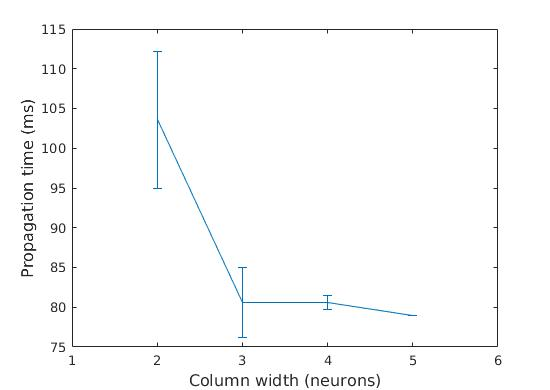
\includegraphics[width=\textwidth]{fig/propagation_time}
\end{figure}

\begin{figure}[p]
 \caption{Typical stimulus and response of a column in the separation property characterization. The stimulus (A) is a Poisson spike train injected onto 30\% of the neurons. The resulting column response is shown in (B).}
 \label{fig:reservoir_response}
 \centering
   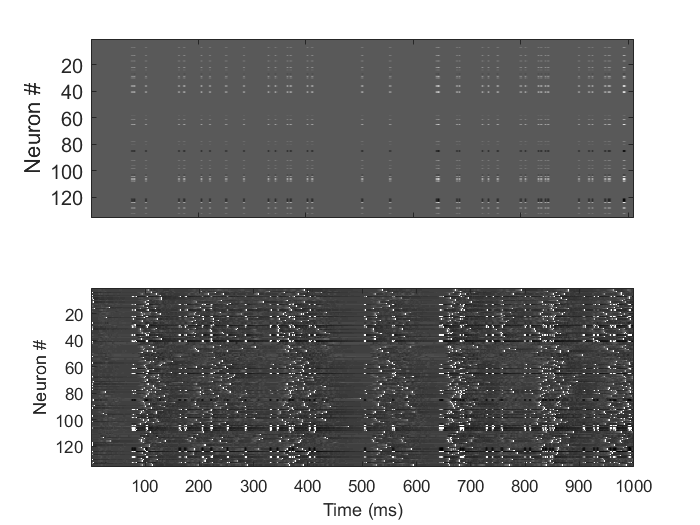
\includegraphics[width=\textwidth]{fig/ReservoirResponse}
\end{figure}

\begin{figure}[p]
 \caption{The neural column trajectories successfully encode the distance between Poisson spike trains.}
 \label{fig:distance}
 \centering
   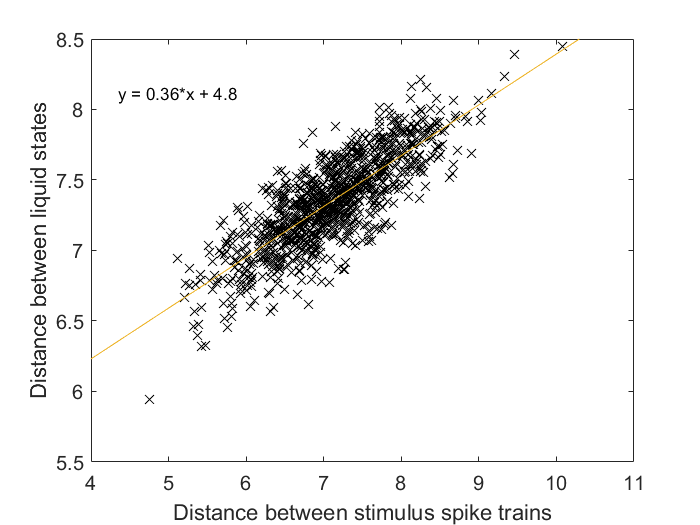
\includegraphics[width=\textwidth]{fig/Distance}
\end{figure}


\clearpage
\printbibliography

\end{document}
